\documentclass[conference]{IEEEtran}
\IEEEoverridecommandlockouts
\usepackage[ngerman]{babel}
% The preceding line is only needed to identify funding in the first footnote. If that is unneeded, please comment it out.
\usepackage{cite}
\usepackage{amsmath,amssymb,amsfonts}
\usepackage{algorithmic}
\usepackage{graphicx}
\usepackage{textcomp}
\usepackage{xcolor}
\usepackage{setspace}
\usepackage{booktabs}
\usepackage[export]{adjustbox}
\def\BibTeX{{\rm B\kern-.05em{\sc i\kern-.025em b}\kern-.08em
    T\kern-.1667em\lower.7ex\hbox{E}\kern-.125emX}}
\begin{document}

\title{Phasen, Techniken und Strategien der Softwareentwicklung an Hand einesKursprojekts im Modul SWE-II}

\author{\IEEEauthorblockN{1\textsuperscript{st} Matz, Annika}
\IEEEauthorblockA{
Berlin, Deutschland \\
s\_matz22@stud.hwr-berlin.de}
\and
\IEEEauthorblockN{2\textsuperscript{nd} Liebenberg, Benjamin}
\IEEEauthorblockA{
Oranienburg, Deutschland \\
s\_liebenberg22@stud.hwr-berlin.de}
\and
\IEEEauthorblockN{3\textsuperscript{rd} Reetz, Tobias}
\IEEEauthorblockA{
Berlin, Deutschland \\
s\_reetz22@stud.hwr-berlin.de}
%Beispiel wie es aussah
%\and
%\IEEEauthorblockN{3\textsuperscript{rd} Given Name Surname}
%\IEEEauthorblockA{\textit{dept. name of organization (of Aff.)} \\
%	\textit{name of organization (of Aff.)}\\
%	City, Country \\
%	email address or ORCID}
}

\maketitle


\section{Disclaimer}
Aus Gründen der besseren Lesbarkeit wird auf die gleichzeitige Verwendung der Sprachformen männlich, weibich und divers (m/w/d) verzichtet. Sämtliche Personenbezeichnungen gelten gleichermaßen für alle Geschlechter.

\section{Einführung}
Innerhalb des dualen Studiums der Informatik an der "Hochschule für Wirtschaft und Recht", fand das Modul Software-Engineering 2 statt. Ziel dieses ist die Entwicklung von Software zu vermitteln und das erlernte Wissen, innerhalb einer Projektarbeit anzuwenden. Dabei wird auf die Grundlagen des Projektmanagments geachtet, wofür z.B. UML-Diagrammen angefertigt werden. Zur Dokumentation des Projektes wird ein Paper angefertigt. 
Innerhalb des Moduls werden auch Softskills gefördert, z.B. die Präsentationsfähigkeiten oder die Sozialkompetenzen innerhalb von Gruppenarbeiten.

\section{Idee des Projektes}
Ein sehr großer Teil unseres Lebens dreht sich um das erwerben von unterschiedlichen Materiellen Gütern. Für unserer Arbeit werden wir vergütet, im Supermarkt kaufen wir davon unser Abendessen und an den Wochenenden und im Urlaub gehen wir auf Reisen. Auf diesen müssen wir uns in einer fremden Kultur zu Recht finden und konsumieren weitere Güter. Doch wie können wir einen Wert von diesen einschätzen, wenn wir die Währung nicht kennen? Genau dieses Problem löst die App "Currency Exchange". Einfaches nachschlagen von tagesaktuellen Wechselkursen und umrechnen zwischen verschiedenen Währungen. Ein besonderes Feature ist das Umwandeln des eingegebenen Wertes in die Anzahl von Döner, welche damit gekauft werden könnten. Dies soll das Gefühl für den Wert des jeweiligen Betrages schulen.\\
Die  Android-App arbeitet mit Hilfe eines Webscrapers, welcher die täglichen Wechselkurse sammelt.


\section{Projektorganisation}
Innerhalb eines Softwareentwicklungsprojekts erhalten die einzelnen Gruppenmitglieder verschiedene Rollen, die ihnen unterschiedliche Aufgaben zu teilen. In diesem Fall bestand das Entwicklungsteam aus drei Personen. So wurden Aufgaben nach und nach vergeben, wobei jeder Bereich eine eigene Ansprechperson besaß. Unterteilt wurde in Projektleitung, Serveradministration, Design und Testdurchführung. Zu Anfang wurde für essentiell wichtige Themen, wie z.B. die Software-Architektur oder den groben Design-Entwurf, Teammeetings durchgeführt und die Umsetzung so zusammen geplant. Sichergestellt wurde so, dass jedes Teammitglied mit einbezogen wird und alle auf dem gleichen Stand sind. \\
Die Programmierung der Software wurde von Teammeeting zu Teammeeting aufgeteilt. Hauptsächlich kümmerten sich Benjamin Liebenberg und Tobias Reetz um die Programmierung des Webscrapers, sowie die Schnittstelle und ein Teil des Backend der App. Annika Matz kümmert sich vor allem um die Umsetzung des Designentwurfs zu einem funktionierenden Frontend, sowie ein Teil der Programmierung des Backend.

\subsection{Projektleitung}
Der Projektleitung wurde von Annika Matz übernommen. Unteranderem behielt sie die unterschiedlichen Abgabetermine im Blick. Außerdem sorgte sie für regelmäßig Treffen in der Gruppe und leitete diese an. Bei diesen wurde der aktuelle Stand ausgewertet, weitere Entwicklungsschritte besprochen und Aufgaben verteilt. \\
Des weiteren achtete sie auch auf die Projektanforderungen und führte die Qualitätssicherung durch, wodurch sie für eine angemessene Feedback innerhalb der Teammeetings sorgt.

\subsection{Serveradministration}
Der Bereich Serveradministration wurde von Benjamin Liebenberg beaufsichtigt. Aufgrund seiner weitreichenden Erfahrung in diesem Gebiet, konnte er diesen Bereich übernehmen. Er hostet unseren Webscraper auf seinem Server, sorgt für täglich aktualisierte Daten innerhalb der App und stellt die Schnittstelle für unsere App bereit.

\subsection{Design \& Testplanung}
Das Design und die Testplanung wurden zum größten Teil von Tobias Reetz übernommen. Aufgrund seiner Designerfahrung im Modul Software-Engineering 1, übernahm er diese Rolle und designte vor allem das App-Logo. Er sorgte für eine angemessene Farbgebung und dafür, dass die App aufgrund ihrer Gestaltung schnell wieder erkennt werden kann. \\
Außerdem übernahm er das Konkretisieren von Usability-Tests, welche wir zuvor im Plemnum entworfen hatte und führte diese mit unseren Kommilitonen durch. Damit trug er einen entscheidenen Beitrag zur Fehlersuche und somit zur Qualität unseres Programmes bei.

\section{Anforderungen}
An eine Software werden immer unterschiedliche Erwartungen und Anforderungen gestellt. Eine genaue Definition sind wichtig für den Erfolg des Projektes. In diesem Projekt werden die unterschiedlichen Anforderung in drei Kategorien unterteilt. Sie beinhalten nicht funktionale, funktionale und optionale funktionale Anforderungen.

\subsection{Nicht funktionale Anforderungen}
Nicht-funktionale Tests decken alle Anforderungen ab, welche das gesamte System ansich betreffen. Es werden somit keine Funktionen abgeprüft, sondern Eigenschaften und Bestandteile. Für das Projekt wurde besonders auf eine sehr gute Usability geachtet, was besonders durch eine intuitive und einfache Benutzung begründet werden soll.
Desweiteren soll eine Verfügbarkeit des Projekt auf Android-Handys garantiert werden. Um einen hohen Datenschutz garantieren zu können erheben wir keine Daten und speichern auch nicht die in der Vergangenheit getätigten Eingaben dem Nutzer zur Verfügung. 

\subsection{Funktionale Anforderungen}
Funktionale Anforderung definieren die Funktionen und Erwartungen der Software, welche für ein erfolgreiches Projekt erfüllt werden müssen. \\
Das wichtigste Ziel für die Software ist eine lauffähige Android-Handy-Applikation, welche verschiedene Eingaben zwischen verschiedenen Währungen richtig Umrechnen kann. Es soll immer ein tagesaktueller Wechselkurs bereit stehen. In die App sollen auch mindestens sieben Währungen eingebunden werden.

\subsection{Optionale funktionale Anforderungen}
Anforderungen, welche nicht essentiell notwendig für die grundlegenden Funktionsweise sind, aber sie diese erweitern, werden zu den optionalen funktionalen Anforderungen gezählt. \\
Zu diesen zählt die Umrechnung der Anzahl an Döner, die die Nutzenden sich mit dem eingetragenen Wert kaufen könnten in Euro. Außerdem könnte die App durch eine Funktion zum Hinzufügen von Prozentualen Werten ergänzt werden. Diese könnten zum Beispiel zur Berechnung der Mehrwertsteuer oder des Trinkgeldes genutzt werden.

\section{Entwurf}
Innerhalb eines Entwurfs wird der Aufbau und die Struktur des Projektes geplant und fest gehalten. Dieser besteht in diesem Projekt aus drei verschiedenen Komponentne der Systemarchitektur, einem Sequenzdiagramm und dem groben Designentwurf der Applikation. Diese Vorgaben dienen als Leitfaden für die Entwicklung der Anwendung.

\subsection{Systemarchitektur}
Die Systemarchitektur beschreibt die Struktur des Projektes, vorhandenen Komponenten und unterschiedlichen Bereiche, während sie zusätzlich erklärt wie diese miteinander interagieren. 
Currency Exchange’s Systemarchitektur besteht aus den zwei Bereichen User-Client und Server. Da hier nur zwei Bereiche existieren handelt es sich um eine Zwei-Tier-Architektur, weil es einen Applikationsbereich also den User-Client und einem Back-End- bzw. Datenbankbereich dem Server besteht.\\
Der User-Client enthält die Business-Logik, welche durch die zwei Unterkategorien View, welcher dabei die Benutzeroberfläche darstellt, und Controller, der für die Verarbeitungslogik die Verantwortung trägt, aufgebaut ist. Der View besteht aus dem Header, der das Logo von Currency Exchange enthält und dem Knopf für den Dark-Mode, der Navigationsleiste, welche eine Übersicht über die verschiedenen Seiten anzeigt, und dem Inhalt, wo dann sämtliche Informationen und Interaktionen statt finden. Über die Interaktion mit diesen können Nutzende mit dem Controller interagieren, über den die unterschiedlichsten Funktionen ausgeführt werden können. Der Controller besteht hier auch wieder aus drei Komponenten. Die erste ist der Navigator, in ihm ist geregelt wie die bereitgestellten Daten formatiert werden sollen, damit sie für die Nutzenden im View beim Inhalt ordnungsgemäß dargestellt werden können. Ein weiterer Teil des Controllers ist der Calculator, welcher für sämtliche Umrechnungen zuständig, wofür er auch Anfragen an den Navigator schickt, um zu wissen welche Operation er durchzuführen hat, und an die letzte Komponente, dem Data-Manager, von dem er die entsprechenden Wechselkurse erfragt. Der Data-Manager ist für die Verarbeitung der Daten zuständig, wozu das Abspeichern, das Einlesen, das Aufarbeiten und Aktualisieren, wofür er per HTTP-Request Anfragen an den Server sendet, der Daten gehört.\\
Der Server beinhaltet auch einen Controller, der aus einem Bash-Skript und einem Data-Manager. Das Bash-Skript ist für den Webscraper verantwortlich, was bedeutet, dass es den Webscraper einmal am Tag aktiviert, welcher dann wiederum Daten aus dem Internet sammelt. Nach dem der Webscraper die Daten gesammelt hat, wird der Data-Manager aktiviert welcher dann diese aufarbeitet und in einer CSV-Datei bereit stellt, da sie eine einfaches Arbeiten durch ihre Strukturierung ermöglicht.\\
Durch die Einbindung des Webscraper auf einem externen Server, wird eine geringe Anfrage auf die Website mit den Wechselkursen garantiert. Denn sollten zu viele Anfragen an die Webseite geschickt werden, kann es zu einer Überlastung dieser kommen. Mögliche folgen wären das Abstürzen dieser Seite.

\subsection{Sequenzdiagramm}
Das Sequenzdiagramm ist für die graphische Darstellung der Kommunikation von den unterschiedlichen Instanzen innerhalb der Software und mit dem User verantwortlich. 
Das Diagramm ist in mehrere Bereiche untergliedert, welche der Serverbereich, Kommunikation von der Applikation und Server und der Interaktion mit dem User sind.
Der Server besteht aus verschiedenen Instanzen, die für die Funktionalitäten verantwortlich sind. Die erste Komponente ist der Webscraper, welcher zur Zweiten, der Webseite von der die Informationen bezogen werden, eine Anfrage schickt, woraufhin diese die Antwort mit sämtlichen Daten zurücksendet. Nach dem Erhalt des Webseiteninhalts, sortiert der Webscraper sämtliche Informationen und sendet sie an die dritte Instanz, welche die Wechselkursliste ist und die die sortierten Daten dann abspeichert.\\
Die Applikation ist eine Instanz innerhalb des Sequenzdiagramms, welches durch die zwei Teilinstazen dem Back- und Front-End vertreten wird und es für die letzten beiden Bereiche des Diagramms verantwortlich ist. Für den Ersten dieser Bereiche ist nur das Back-End verantwortlich, weil es an den Server, genauer gesagt an die Währungsliste, eine Anfrage sendet, mit der die aktualisierten Daten abgefragt werden sollen. Besteht eine Internetverbindung sendet die Liste die neuen Informationen an das Back-End, welches dann die Informationen intern abspeichert. Sollte jedoch keine Verbindung zum Internet bestehen wird mit den schon besthenden Daten der Applikation weiter gearbeitet.\\
Innerhalb des letzten Bereiches des Diagramms, welcher sich mit der Verarbeitung der der User-Inputs beschäftigt, spielen auch die Instanzen des Font-Ends und des Users eine Rolle. Der User hat diverse Möglichkeiten mit der Applikation zu interagieren, welche in die zwei Kategorien , die jeweils einen ähnlichen Aufbau aufweisen, der logischen und graphischen Anpassung unterteilt werden kann.  Bei der logistischen Komponente sendet der User eine von drei Nachrichten an das Back-End, welches dann eine Anfrage über die ausgewählten Werte an das Front-End sind. Die Userbefehle sind klickSwapSpinnerValues, welche die ausgewählten Währungen miteinander tauscht, selectCurrency, welche es ermöglicht eine neue Währung auszuwälen, und klickCalculateValues, welche die Werte berechnet. Nach dem Erhalt der Informationen des Front-Ends, führt das Back-End dann jeweils Funktionen aus, die die Werte tauschen, neue aus wählen oder den Wechselkurs und die Döneranzahl berechnen. Zum Schluss sendet es die Berechnungen zurück an das Front-End, welches daraufhin das Anzeigen dieser übernimmt. Die letzten drei Möglichkeiten, die der User hat, sind die graphischen Anpassen, bei denen entweder die Home-Seite  oder die FAQ-Seite angzeigt wird und zwischen Dark- und Light-Mode gwechselt werden kann. Dafür sendet der User eine Nachricht an das Front-End, welches dann die Veränderungen darstellt.

\subsection{grober Designentwurf}
Abbildung \ref{fig:designentwurf} zeigt den vorläufigen Entwurf des Designs. Er besteht, wie in der Softwarearchitektur beschrieben, aus einem Header, Inhalt und Navigationsleiste. Der Header ist oben im Bild zuerkennen und zeigt das Logo von Currency Exchange auf. Dieses wurde mit einem weißen Kreis hinterlegt und so hervorgehoben, um einen Kontrast zu dem immer wieder kehrenden Hellblau zu kreieren. Auch im Inhalt ist das Blau als Schrift und Hervorhebung wieder zu finden, weil durch das immer wieder kehrende Farbschema, soll eine Konsistenz erschaffen werden, welche die Nutzenden davon überzeugen soll sich immer wieder auf die Applikation verlassen zu können. Der Hintergrund wurde zusätzlich in einem Grauton dargestellt, um von den wesentlichen Inhalten nicht abzulenken und wodurch auch noch einmal das Farbschema unterstützt werden soll. Die Navigationsleiste wird durch die drei vertikalen Striche oben links im Bild angedeutet, weil sie aus platztechnischen Gründen erst bei einer Interaktion mit den Strichen von der Seite erscheint. In der Navigation wird auch das blau-weiße Farbschema verwendet, welches sich natürlich auch in der FAQ-Seite wieder findet.
\begin{figure}[h]
	\centering
	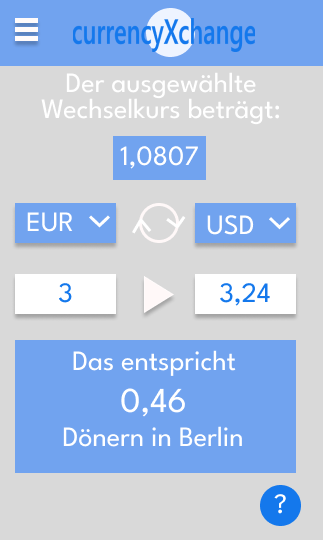
\includegraphics[width=0.5\linewidth, frame]{designentwurf}
	\caption[Designentwurf]{Designentwurf}
	\label{fig:designentwurf}
\end{figure}

\section{Implementierung}

\subsection{Konsistenz}
Ein wichtiger Punkt bei der Implementierung ist die Konsistenz, welche beschreibt, dass die Daten ihre Richtigkeit haben. Die Informationen über die Wechselkurse, werden von der Webseite aus Quelle \cite{waechselkurse} bezogen. 

\subsection{Vorbereitung}
Innerhalb der Vorbereitungsphase werden wichtige Punkte für den Verlauf des Projekts festgelegt. Einer dieser Punkte ist die Versionsverwaltung. Über sie werden die verschiedenen Stände der Software gesteuert und überblickt. So kann im Fall von irreversiblen Fehlern auf frühere, lauffähige Versionen zugegriffen werden. Dies ermöglicht einen effizienten Arbeitsflow. Zu dem ist GitHub kostenfrei und weit verbreitet, was bei Problemen mit der Versionsverwaltung zu einem breiten Angebot von Hilfestellungen und eine große Community führt.\\
Ein weiterer Punkt ist die Namenskonvention von Funktionen, Variablen und Dateien. Hierbei wurde festgelegt, dass die Namen deskriptiv sein sollen, damit sie möglichst einfach zu verstehen sind. Deskriptive Namen werden so gestalten, dass der Namen alleine die Funktionalität beschreiben kann, wodurch viele Kommentarzeilen eingespart werden können. Dabei übernimmt der Name dieser Funktion die Erklärung, was innerhalb passiert und sollte selbst erklärend benannt sein.\\
Einer der wichtigste Punkte innerhalb der Entwicklung einer Software ist die verwendete Programmiersprache und Entwicklungsumgebung. Das Ziel bei Currency Exchange ist unteranderem die Darstellung in einer Android-App. Bei der Suche nach einer passenden Entwicklungsumgebung wurde vor allem darauf geachtet, dass sie den Entwicklungsprozess durch Verbesserungsvorschläge und graphische Darstellungen der Applikation unterstützt. Eine solche Entwicklungsumgebung ist Android-Studio, weil sie ohne weitere Einstellungen Codeverbesserungen vorschlägt und einen eingebauten Emulator besitzt. Dieser vereinfacht es die Anwendung graphisch wahrzunehmen, zu simulieren und Fehler während der Laufzeit zu finden. Zusätzlich wird dies auch durch die Namensgebung der Entwicklungsgebung unterstrichen. Innerhalb von Android-Studio besteht die Möglichkeit zwischen den zwei Programmiersprachen Kotlin und JAVA zu wählen, welche beide objektorientierte Sprachen sind. Durch die bereits vorhandenen Vorkenntnisse des Projektteams mit der Programmiersprache JAVA, wurde sie als Entwicklungssprache ausgewählt. Somit war keine weitere Einarbeitung in eine neue Sprache nötig und es konnte direkt mit der Entwicklung der Applikation begonnen werden. Neben der Anwendung muss auch eine Programmiersprache für den Webscraper ausgewählt werden. Für diesen wurde die Sprache C\# gewählt, da Benjamin Liebenberg bereits einen Webscraper in dieser Programmiersprache erstellt hatte. Dies ermöglichte eine Zeitersparnis, weil auch hier keine Einarbeitung in eine neue Programmiersprache statt finden musste. Des Weiteren ist C\# sicherer und skalierbarer bei Webservices als JAVA (vgl. S. 11 \cite{csharpperformance}) und C\# kann auch Plattform unabhängig agieren.

\section{Integration}
Die Integration in der Softwareentwicklung beschäftigt sich mit den Schnittstellen zwischen den unterschiedlichen Systemkomponenten und der Testung dieser. Es ist wichtig, dass diese miteinander kompatibel sind und bei den Übertragungen der zwischen Komponenten keine Fehler auftreten. Hierzu stehen den entwickelnden Personen diverse Methoden zur Verfügung. Eine von diesen ist die Top-Down Integration. Sie kennzeichnet sich dadurch aus, das die obere Schichten zu erst integriert werden. Dabei werden die unteren Schichten durch Simulationen dargestellt. Dies ermöglicht das Testen der Grundfunktionalitäten zu erst, bevor dann im darauffolgenden Schritt die Komponenten zusammengeführt und erneut überprüft werden.\\
Im Fall von Currency Exchange bedeutete dies, dass im ersten Schritt der User-Client, welcher mit Hilfe von fest eingebauten Werten getestet wurde, und der Webscraper, der die CSV-Datei über einen Port zugänglich macht und überprüft wurde, ob alle Daten richtig sortiert wurden, integriert. Im zweiten Schritt wurde die beiden Komponenten zusammen geführt und bildeten ein neues System, welches dann erneut überarbeitet und getestet worden ist. \\
Es wurde auch überlegt diverse andere Integrationsstrategien zu verfolgen wie zum Beispiel den Big-Bang Methode, allerdings bat sie sich nicht an, weil sie sämtliche Komponenten mit einem Schritt integriert, was zur Folge hat, dass im Nachhinein der Debuggingaufwand wesentlich erhöht gewesen wäre, weil es sich bei Currency Exchange um eine neue Software handelt, bei der es sich anbietet ein iteratives Vorgehen zu wählen, da somit die neu erstellten Komponenten ausgetestet werden können.

\section{Tests}
Um zu validieren, dass die Software in ihren Funktionen korrekt ist, muss diese ausreichend getestet werden. Dazu sollten die Funktionen, die Persistenz und die Handhabung überprüft werden. Um dies zu bewerkstelligen, wird von Testmethoden Gebrauch gemacht. Da es jedoch kaum möglich ist, alle Bestandteile der Software gleichzeitig zu testen, wird die Überprüfung in mehrere Schichten unterteilt.\\
Während der Implementierungsphase, also der eigentlichen Entwicklung der Applikation, wird hierzu auf das Experience-based Testing zurückgegriffen. Bei dieser Art des Testens wird die Testtiefe durch individuelle Erfahrungen erzeugt. Dadurch entstehen potenziell verschiedene Tests mit unterschiedlichen Teststärken. Der größte Vorteil davon ist, dass besonders erfahrene Personen einen Fehler finden könnten, der bei konventionellen Methoden unentdeckt bleiben würde. Somit kann der Entwickler Fehler direkt ausfindig machen und möglichst unmittelbar an der Behebung dieser arbeiten.\\
Jedoch birgt diese Testmethode auch Risiken. Schließlich kann es vorkommen, dass auf einem Gebiet keine Expertise vorhanden ist, wodurch Fehler unentdeckt bleiben. Aus diesem Grund wurde während der Erstellung der Software zusätzlich auf das sogenannte Beta-Testing zurückgegriffen. Dabei wird die Applikation von Personen getestet, welche mit den Funktionen und der Benutzeroberfläche nicht vertraut sind. Dadurch kann es zu einer Fehlbedienung kommen, welche aus Sicht der Entwickler im schlechtesten Falle zu einem Absturz des Programms führt, im besten Fall nur einen Fehler auswirft. Außerdem füllen die Personen nach dem Testen der Applikation einen kurzen Fragebogen aus, welcher vor allem die Dokumentation der Fehler und Anregungen für etwaige Verbesserungen zum Thema hat. Sinngemäß beinhaltet das Beta-Testing also die Testmethoden für die Benutzerfreundlichkeit (eng. usability-tests), als auch für die Funktionalitäts-Tests (Black-Box-Testing). Mit diesen gewonnen Daten kann die Anwendung anschließend verbessert  und mögliche Fehler beseitigt werden. \\
Im Fall von Currency Exchange wurde ein Beta-Test am 13.03.2024 durchgeführt, welcher aufschlussreiche Informationen über die Verbesserung der Applikation geliefert hat. Beispielsweise wurden einige Fehler gefunden, die den Absturz der Software zur Folge hatten. Ein solcher Fehler trat bei der Umrechnung gleicher Währungen auf. Dieser konnte durch das gezielte Abfangen der Operation behoben werden. Ein weiterer schwerwiegender Fehler tritt auf, wenn der Nutzer den Dark-Mode-Schalter verwendet, während er sich auf der Informationsseite befindet. Die Ursache wurde zeitnah ermittelt, allerdings konnte der Fehler noch nicht behoben werden. Hauptgrund hierfür ist die Komplexität des Quellcodes innerhalb der .xml-Dateien, welche primär für das Anzeigen der Benutzeroberfläche zuständig sind.\\
Neben den technischen Problemen wurden Anregungen hinsichtlich der Benutzeroberfläche und Bedienung getätigt, welche eine Überarbeitung des Designs zur Folge hatten. Beispielsweise wurde angemerkt, dass die Währungen in scheinbar willkürlicher Reihenfolge vorlagen, wobei sie eigentlich alphabetisch nach den Ländernamen sortiert wurden. Um eine bessere Benutzung zu gewährleisten, wurden die Währungen deshalb absteigend nach ihrem Währungsnamen geordnet. Hierbei befinden sich die üblichen Währungen, wie US-Dollar, Yen, Euro und Hongkong-Dollar, aus Gründen der Verwendungshäufigkeit am Anfang der Liste. 

\section{Rollout}
Nachdem die Tests erfolgreich ausgeführt wurden, kann es zum Rollout der Applikation kommen. Zum Zeitpunkt der Erstellung des Papers ist noch keine Veröffentlichung geplant, weshalb keine konkreten Pläne zum Rollout bestehen. \\
Allerdings wird die Software lokal betrieben, um weitere Veränderungen vorzunehmen und die Anwendung so Stück für Stück zu verbessern. Um die Applikation also weiter betreiben zu können, ist die Schnittstelle zum Webserver immer noch von Bedeutung. Hierbei wird der Server über den Anbieter „Strato“ gemietet. Die Quelldateien des Webscrapers zum Abrufen der Wechselkurse wurden hierzu auf dem Server abgelegt und anschließend eine binäre Datei daraus gebaut. Daraufhin wurde ein Script für diese Binärdatei erstellt, um diese beim Aufruf des Scriptes auszuführen. Um den Prozess vollständig zu automatisieren, wurde anschließend ein Cron-Job auf dem Server konfiguriert, welcher zu einer voreingestellten Tageszeit das Startscript des Webscrapers aufruft. Dies gewährleistet, dass täglich eine aktuelle Version der Wechselkurse verfügbar ist. Um die Datei nun von Server abrufen zu können, wird die Datei nach dem Aufrufen des Scriptes in einen Unterordner verschoben. \\
Dieser ist mithilfe von Apache so eingestellt, dass man über den Aufruf einer speziellen URL automatisch die abgelegte Datei herunterlädt. Die Applikation selbst wird mithilfe einer .APK-Datei installiert. Hierzu wird die APK von Android-Studio gebaut und dann mithilfe eines Datenkabels oder via Internet auf das gewünschte Gerät übertragen. Auf dem Smartphone kann die Datei im Anschluss durch einen einfachen Klick
geöffnet werden, woraufhin ein Dialog zum Installieren der Applikation erscheint. Dies ist jedoch nur dann möglich, wenn zuvor in den Einstellungen konfiguriert wurde, dass fremde oder unbekannte Dateien installiert werden dürfen. Hauptgrund hierfür ist vor allem, dass die Applikation nicht offiziell lizenziert wurde. \\
Nachdem die Installation abgeschlossen wurde, kann die App einfach geöffnet werden. Hierbei ist zu beachten, dass beim Erststart eine Internetverbindung verfügbar ist, damit eine aktuelle Version der Wechselkurse heruntergeladen wird. Versucht man die Applikation zu starten, ohne das eine Internetverbindung vorhanden ist, so schließt sich die App direkt, da keine valide Datei für die Wechselkurse gefunden werden kann. Bei späteren Benutzungen ist es nicht mehr notwendig, die App mit einer verfügbaren Internetverbindung zu nutzen, da zumindest eine Datei mit Wechselkursen verfügbar ist. Möchte die nutzende Person jedoch sicherstellen, dass immer die aktuellen Wechselkurse auf dem Gerät verfügbar sind, so muss beim ersten Start eines jeden Tages sichergestellt werden, 
dass eine Verbindung zum Internet besteht.

\section{Wartung}
In der internationalen Norm für Software-Lebenszyklusprozesse (ISO / IEC 12207), sind vor allem die Hauptpunkte Inbetriebnahme und Wartung als besonders wichtig hervorgehoben.
Demnach beschäftigt sich die Inbetriebnahme der Software vor allem mit der Systemeinführung und -überprüfung sowie der Unterstützung der Benutzenden. Würde es also zu einem Rollout kommen, so müsste man auch sicherstellen, dass den Nutzenden bei der Verwendung der Applikation genügend Unterstützungen entgegen gebracht wird. Hierzu wurde eine Informationsseite innerhalb der Applikation angefertigt, auf welcher sich der Nutzer über die Handhabung der einzelnen Funktionen informieren kann. \\
Des Weiteren ist eine kontinuierliche Wartung der Software nach dem Release erforderlich. Hierzu wird die Wartung in verschiedene Arten unterteilt: 
Die adaptive Wartung beschäftigt sich beispielsweise mit der Anpassung der Software an verschiedene Anforderungen. So soll die App im Fall von Currency Exchange auf den verschiedensten Bildschirmgrößen verfügbar sein und automatisch skalieren. Darüber hinaus werden in diesem Teil der Wartung auch weitere Features implementiert. Zu einem solchen Feature zählt etwa das Anzeigen der vergangenen Wechselkurse beziehungsweise eine Statistik über die Wertentwicklung der einzelnen Währungen. Außerdem ist auch die Bereitstellung für andere Betriebssysteme von Relevanz. So ist insbesondere das Ziel, die App für IOS bereitzustellen und damit potentielle Nutzende anzuwerben.\\
Eine andere Art der Wartung ist die präventive Wartung. Bei dieser Art steht die Fehlervorbeugung im Vordergrund. Wird eine neuere Version des Betriebssystems veröffentlicht, so können verwendete Methoden veralten, wodurch die Funktionalität nicht mehr gegeben wäre und die Software womöglich unbrauchbar wird. Mit der ständigen Überwachung und Verbesserung des Quellcodes kann dem vorgebeugt werden. \\
Sollte zu einem Zeitpunkt auffallen, dass die Verarbeitungsdauer der einzelnen Prozesse zu lange dauert, so wäre dies ein Fall für die verbessernde Wartung. Hierbei soll der Quellcode so optimiert werden, dass sich die Berechnungszeit verringert, die Reaktionszeit verbessert und die App somit performanter arbeitet. Da Currency Exchange keine Nutzungsdaten erhebt, kann dies nur durch eigene Tests ermittelt werden. Hierzu liegen jedoch noch keine ausreichenden Daten vor.\\
Die letzte Art der Wartung ist die korrektive Wartung. Bei dieser geht es insbesondere um die Behebung bekannter Fehler, um zum Beispiel den Absturz der Applikation zu vermeiden. Auch bei Currency Exchange muss diese Wartungsart angewandt werden, da auch in der aktuellen Version Fehler existieren, die schwerwiegende Fehler produzieren können, welche direkt zur Beendung der App führen. Ein bekannter Fehler ist beispielsweise der Wechsel vom Dark-Mode in den Light-Mode innerhalb der Info-Seite, welcher unmittelbar nach Betätigung des Knopfes zum Schließen der Applikation führt. Die Ursache für diesen Fehler konnte durch ausgiebige Tests ermittelt werden und in zukünftigen . 

\section{Ergebnis}
Die entwickle Software läuft bis auf vereinzelte Ausnahmen komplikationslos und erfüllt alle Grundanforderungen, sowie vereinzelt optionale funktionale Anforderungen. Darunter fällt die Berechnung in Döner.  Das Abziehen bzw. Hinzufügen von prozentualen Anteilen konnte nicht umgesetzt werden. Die Grundanforderung, dass mindestens 7 Währungen angeboten werden sollen, konnten mit etwa 140 verschiedenen Währungen bei weitem übertroffen werden.\\
Herausforderungen brachte vor allem das Design des Frontends der App. Während der Implementierung wurde festgestellt, dass einige Funktionen innerhalb der Benutzeroberfläche fehlen. Manche führten jedoch zu einer sehr überladenen und unübersichtlichen Oberfläche. Auf Grundlage dessen wurden Funktionen wieder entfernt. So kam über die weitere Entwicklung der App eine textliche Anzeige der umgerechneten Werte hinzu. Diese soll die Bedeutung der einzelnen Werte verdeutlichen und für eine bessere Verständlichkeit sorgen. Dadurch wurde die Benutzeroberfläche sehr voll, wodurch einige Elemente entfernt werden musste. Ein solches Element war der Info-Knopf, über den die Nutzenden Informationen zur Bedienung der Anwendung erhalten konnten. Da dies lediglich eine Alternative zum Informationstext war, welchen man über die Navigationsleiste im Hamburger-Menü erreichen konnte, war der Knopf obsolet. \\
Mit der fortschreitenden Implementierung weiterer Währungen, entstand eine unübersichtliche Liste, welche die Auswahl beim Suchen einer speziellen Währung zeitlich stark intensivierte. Um dieses Problem zukünftig zu lösen, könnte eine Suchfunktion integriert werden. Als Unterstützung der Nutzenden wurde vorerst eine Art der Sortierung vorgenommen, bei der zuerst die üblichen Währungen aufgelistet sind und anschließend eine alphabetische absteigende Reihenfolge nach Währungsnamen folgt. \\
Durch immer wiederkehrende Verbesserungsmöglichkeiten hinsichtlich der Nutzeroberfläche konnte die Gruppe ihre Kompetenzen in der Front-End Entwicklung weiter ausbauen.

\section{Abschluss}
Das Projekt konnte erfolgreich abgeschlossen werden. Die Fähigkeiten innerhalb der Software Entwicklung wurde weiter vertieft und ausgebaut. Weiterhin konnte eine lauffähige Software mit allen funktionalen Anforderungen entwickelt werden.
Besonders gut verlief die Arbeit innerhalb der Teammeetings. Es gab dauerhaft eine konstruktive Arbeitsatmosphäre, in welcher vor allem während der Phase der Konzeptionierung zielgerichtet diskutiert werden konnte. Fehler wurden in der Gruppe besprochen und gemeinsam behoben, wodurch ein schneller Lösungsansatz erarbeitet wurde.\\
Trotzdem traten vereinzelt Schwierigkeiten in der Kommunikation während der Implementierungsphase auf. So entstanden Situationen, in welchen es bei den Gruppenmitgliedern zu einer Fehlkommunikation kam oder teils wichtige Informationen verloren gegangen sind. Insbesondere konnte dies jedoch durch die vielen Gruppenmeetings und Absprachen schnell behoben beziehungsweise korrigiert werden, sodass keine größeren Diskrepanzen innerhalb der Gruppe entstanden sind. Durch diese Erfahrungen konnten wir unsere Softskills innerhalb der Kommunikation untereinander verbessern. Im Bereich der Gruppenkommunikation haben die Teammitglieder über die Zeit hinweg ihre Fähigkeiten in Bezug auf die Informationsvermittlung verbessert.\\
Insgesamt konnte das Softwareprojekt erfolgreich abgeschlossen werden. Vor allem in Hinblick auf fachliche Kompetenzen konnten sich die einzelnen Gruppenmitglieder weiter entwickeln und neue Erfahrungen sammeln. Schwierige Situationen konnten auf Basis einer sehr guten internen Kommunikation gemeistert werden.


\begin{thebibliography}{99}
	\bibitem[1]{csharpperformance}
	Sagayaraj, S., and M. Santhosh Kumar. "Performance evaluation of web services in C\#, JAVA, and PHP."\space International Journal of Computer Science and Business Informatics 7.1 (2013).
	\bibitem[2]{waechselkurse}
	Webseite WährungsRechner.de: \\https://www.waehrungsrechner.de/wechselkurse/
\end{thebibliography}

\end{document}
